% Options for packages loaded elsewhere
\PassOptionsToPackage{unicode}{hyperref}
\PassOptionsToPackage{hyphens}{url}
\PassOptionsToPackage{dvipsnames,svgnames,x11names}{xcolor}
%
\documentclass[
  11pt,
]{article}

\usepackage{amsmath,amssymb}
\usepackage{iftex}
\ifPDFTeX
  \usepackage[T1]{fontenc}
  \usepackage[utf8]{inputenc}
  \usepackage{textcomp} % provide euro and other symbols
\else % if luatex or xetex
  \usepackage{unicode-math}
  \defaultfontfeatures{Scale=MatchLowercase}
  \defaultfontfeatures[\rmfamily]{Ligatures=TeX,Scale=1}
\fi
\usepackage{lmodern}
\ifPDFTeX\else  
    % xetex/luatex font selection
    \setmainfont[]{Times New Roman}
\fi
% Use upquote if available, for straight quotes in verbatim environments
\IfFileExists{upquote.sty}{\usepackage{upquote}}{}
\IfFileExists{microtype.sty}{% use microtype if available
  \usepackage[]{microtype}
  \UseMicrotypeSet[protrusion]{basicmath} % disable protrusion for tt fonts
}{}
\makeatletter
\@ifundefined{KOMAClassName}{% if non-KOMA class
  \IfFileExists{parskip.sty}{%
    \usepackage{parskip}
  }{% else
    \setlength{\parindent}{0pt}
    \setlength{\parskip}{6pt plus 2pt minus 1pt}}
}{% if KOMA class
  \KOMAoptions{parskip=half}}
\makeatother
\usepackage{xcolor}
\usepackage[margin=1in]{geometry}
\setlength{\emergencystretch}{3em} % prevent overfull lines
\setcounter{secnumdepth}{-\maxdimen} % remove section numbering
% Make \paragraph and \subparagraph free-standing
\makeatletter
\ifx\paragraph\undefined\else
  \let\oldparagraph\paragraph
  \renewcommand{\paragraph}{
    \@ifstar
      \xxxParagraphStar
      \xxxParagraphNoStar
  }
  \newcommand{\xxxParagraphStar}[1]{\oldparagraph*{#1}\mbox{}}
  \newcommand{\xxxParagraphNoStar}[1]{\oldparagraph{#1}\mbox{}}
\fi
\ifx\subparagraph\undefined\else
  \let\oldsubparagraph\subparagraph
  \renewcommand{\subparagraph}{
    \@ifstar
      \xxxSubParagraphStar
      \xxxSubParagraphNoStar
  }
  \newcommand{\xxxSubParagraphStar}[1]{\oldsubparagraph*{#1}\mbox{}}
  \newcommand{\xxxSubParagraphNoStar}[1]{\oldsubparagraph{#1}\mbox{}}
\fi
\makeatother

\usepackage{color}
\usepackage{fancyvrb}
\newcommand{\VerbBar}{|}
\newcommand{\VERB}{\Verb[commandchars=\\\{\}]}
\DefineVerbatimEnvironment{Highlighting}{Verbatim}{commandchars=\\\{\}}
% Add ',fontsize=\small' for more characters per line
\usepackage{framed}
\definecolor{shadecolor}{RGB}{241,243,245}
\newenvironment{Shaded}{\begin{snugshade}}{\end{snugshade}}
\newcommand{\AlertTok}[1]{\textcolor[rgb]{0.68,0.00,0.00}{#1}}
\newcommand{\AnnotationTok}[1]{\textcolor[rgb]{0.37,0.37,0.37}{#1}}
\newcommand{\AttributeTok}[1]{\textcolor[rgb]{0.40,0.45,0.13}{#1}}
\newcommand{\BaseNTok}[1]{\textcolor[rgb]{0.68,0.00,0.00}{#1}}
\newcommand{\BuiltInTok}[1]{\textcolor[rgb]{0.00,0.23,0.31}{#1}}
\newcommand{\CharTok}[1]{\textcolor[rgb]{0.13,0.47,0.30}{#1}}
\newcommand{\CommentTok}[1]{\textcolor[rgb]{0.37,0.37,0.37}{#1}}
\newcommand{\CommentVarTok}[1]{\textcolor[rgb]{0.37,0.37,0.37}{\textit{#1}}}
\newcommand{\ConstantTok}[1]{\textcolor[rgb]{0.56,0.35,0.01}{#1}}
\newcommand{\ControlFlowTok}[1]{\textcolor[rgb]{0.00,0.23,0.31}{\textbf{#1}}}
\newcommand{\DataTypeTok}[1]{\textcolor[rgb]{0.68,0.00,0.00}{#1}}
\newcommand{\DecValTok}[1]{\textcolor[rgb]{0.68,0.00,0.00}{#1}}
\newcommand{\DocumentationTok}[1]{\textcolor[rgb]{0.37,0.37,0.37}{\textit{#1}}}
\newcommand{\ErrorTok}[1]{\textcolor[rgb]{0.68,0.00,0.00}{#1}}
\newcommand{\ExtensionTok}[1]{\textcolor[rgb]{0.00,0.23,0.31}{#1}}
\newcommand{\FloatTok}[1]{\textcolor[rgb]{0.68,0.00,0.00}{#1}}
\newcommand{\FunctionTok}[1]{\textcolor[rgb]{0.28,0.35,0.67}{#1}}
\newcommand{\ImportTok}[1]{\textcolor[rgb]{0.00,0.46,0.62}{#1}}
\newcommand{\InformationTok}[1]{\textcolor[rgb]{0.37,0.37,0.37}{#1}}
\newcommand{\KeywordTok}[1]{\textcolor[rgb]{0.00,0.23,0.31}{\textbf{#1}}}
\newcommand{\NormalTok}[1]{\textcolor[rgb]{0.00,0.23,0.31}{#1}}
\newcommand{\OperatorTok}[1]{\textcolor[rgb]{0.37,0.37,0.37}{#1}}
\newcommand{\OtherTok}[1]{\textcolor[rgb]{0.00,0.23,0.31}{#1}}
\newcommand{\PreprocessorTok}[1]{\textcolor[rgb]{0.68,0.00,0.00}{#1}}
\newcommand{\RegionMarkerTok}[1]{\textcolor[rgb]{0.00,0.23,0.31}{#1}}
\newcommand{\SpecialCharTok}[1]{\textcolor[rgb]{0.37,0.37,0.37}{#1}}
\newcommand{\SpecialStringTok}[1]{\textcolor[rgb]{0.13,0.47,0.30}{#1}}
\newcommand{\StringTok}[1]{\textcolor[rgb]{0.13,0.47,0.30}{#1}}
\newcommand{\VariableTok}[1]{\textcolor[rgb]{0.07,0.07,0.07}{#1}}
\newcommand{\VerbatimStringTok}[1]{\textcolor[rgb]{0.13,0.47,0.30}{#1}}
\newcommand{\WarningTok}[1]{\textcolor[rgb]{0.37,0.37,0.37}{\textit{#1}}}

\providecommand{\tightlist}{%
  \setlength{\itemsep}{0pt}\setlength{\parskip}{0pt}}\usepackage{longtable,booktabs,array}
\usepackage{calc} % for calculating minipage widths
% Correct order of tables after \paragraph or \subparagraph
\usepackage{etoolbox}
\makeatletter
\patchcmd\longtable{\par}{\if@noskipsec\mbox{}\fi\par}{}{}
\makeatother
% Allow footnotes in longtable head/foot
\IfFileExists{footnotehyper.sty}{\usepackage{footnotehyper}}{\usepackage{footnote}}
\makesavenoteenv{longtable}
\usepackage{graphicx}
\makeatletter
\newsavebox\pandoc@box
\newcommand*\pandocbounded[1]{% scales image to fit in text height/width
  \sbox\pandoc@box{#1}%
  \Gscale@div\@tempa{\textheight}{\dimexpr\ht\pandoc@box+\dp\pandoc@box\relax}%
  \Gscale@div\@tempb{\linewidth}{\wd\pandoc@box}%
  \ifdim\@tempb\p@<\@tempa\p@\let\@tempa\@tempb\fi% select the smaller of both
  \ifdim\@tempa\p@<\p@\scalebox{\@tempa}{\usebox\pandoc@box}%
  \else\usebox{\pandoc@box}%
  \fi%
}
% Set default figure placement to htbp
\def\fps@figure{htbp}
\makeatother

\makeatletter
\@ifpackageloaded{caption}{}{\usepackage{caption}}
\AtBeginDocument{%
\ifdefined\contentsname
  \renewcommand*\contentsname{Table of contents}
\else
  \newcommand\contentsname{Table of contents}
\fi
\ifdefined\listfigurename
  \renewcommand*\listfigurename{List of Figures}
\else
  \newcommand\listfigurename{List of Figures}
\fi
\ifdefined\listtablename
  \renewcommand*\listtablename{List of Tables}
\else
  \newcommand\listtablename{List of Tables}
\fi
\ifdefined\figurename
  \renewcommand*\figurename{Figure}
\else
  \newcommand\figurename{Figure}
\fi
\ifdefined\tablename
  \renewcommand*\tablename{Table}
\else
  \newcommand\tablename{Table}
\fi
}
\@ifpackageloaded{float}{}{\usepackage{float}}
\floatstyle{ruled}
\@ifundefined{c@chapter}{\newfloat{codelisting}{h}{lop}}{\newfloat{codelisting}{h}{lop}[chapter]}
\floatname{codelisting}{Listing}
\newcommand*\listoflistings{\listof{codelisting}{List of Listings}}
\makeatother
\makeatletter
\makeatother
\makeatletter
\@ifpackageloaded{caption}{}{\usepackage{caption}}
\@ifpackageloaded{subcaption}{}{\usepackage{subcaption}}
\makeatother

\usepackage{bookmark}

\IfFileExists{xurl.sty}{\usepackage{xurl}}{} % add URL line breaks if available
\urlstyle{same} % disable monospaced font for URLs
\hypersetup{
  pdftitle={5513Assignment2- Git \& GitHub Beginner's Guide with RStudio and CLI},
  pdfauthor={Jingyi Wang 35678925},
  colorlinks=true,
  linkcolor={blue},
  filecolor={Maroon},
  citecolor={Blue},
  urlcolor={Blue},
  pdfcreator={LaTeX via pandoc}}


\title{5513Assignment2- Git \& GitHub Beginner's Guide with RStudio and
CLI}
\author{Jingyi Wang 35678925}
\date{}

\begin{document}
\maketitle

\renewcommand*\contentsname{Table of contents}
{
\hypersetup{linkcolor=}
\setcounter{tocdepth}{3}
\tableofcontents
}

\section{Introduction}\label{introduction}

This guide demonstrates how to efficiently use Git, GitHub, and the
command line interface (CLI) for version control and collaboration. By
following these steps, you'll master Git for Quarto projects in RStudio.

\section{Step 1: Create a new RStudio Project and a simple Quarto
file}\label{step-1-create-a-new-rstudio-project-and-a-simple-quarto-file}

First, open RStudio and create a new project named
\texttt{5513Assignment2} (Figure~\ref{fig-R_project}).

\begin{figure}

\centering{

\pandocbounded{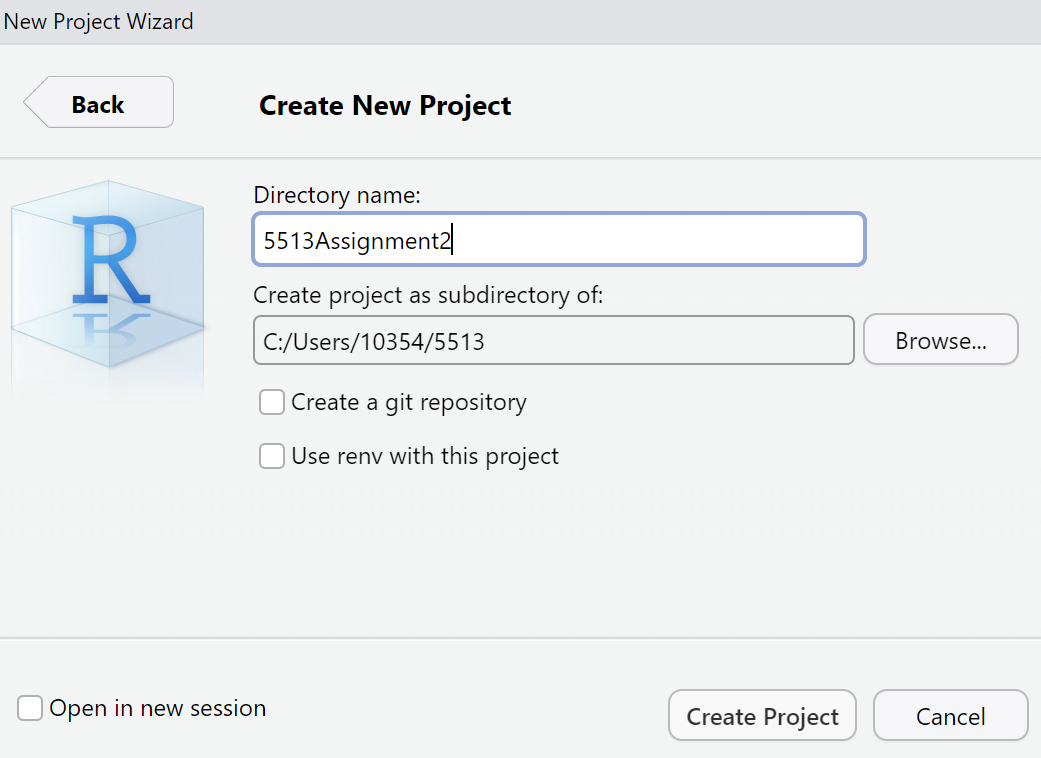
\includegraphics[keepaspectratio]{figure/R_project.png}}

}

\caption{\label{fig-R_project}Create a new R Project}

\end{figure}%

Inside the project, make a new Quarto document called
\texttt{example.qmd} (Figure~\ref{fig-ex_qmd}). Add some simple content
(Figure~\ref{fig-wri_ex_qmd}) and click the Render button to knit it
into an HTML file (Figure~\ref{fig-ex_html}).

\begin{figure}

\centering{

\pandocbounded{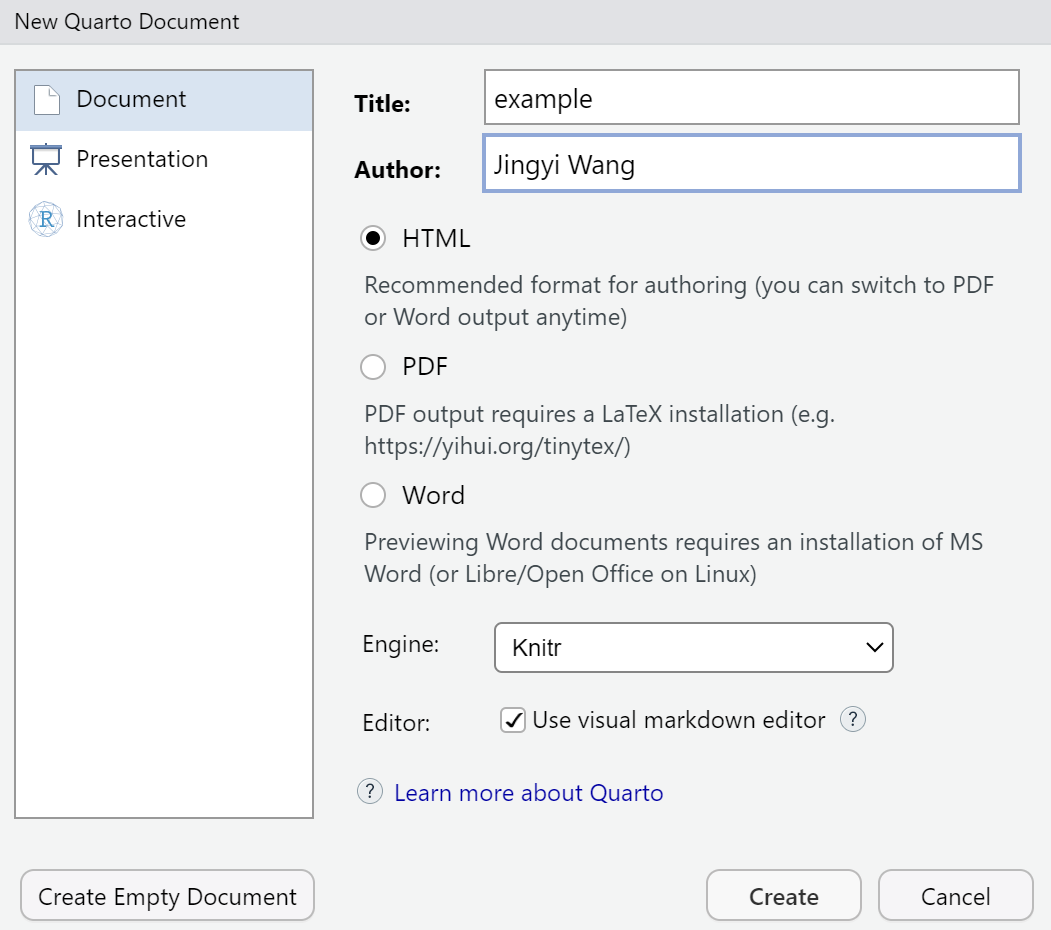
\includegraphics[keepaspectratio]{figure/ex_qmd.png}}

}

\caption{\label{fig-ex_qmd}Create a new Quarto Document}

\end{figure}%

\begin{figure}

\centering{

\pandocbounded{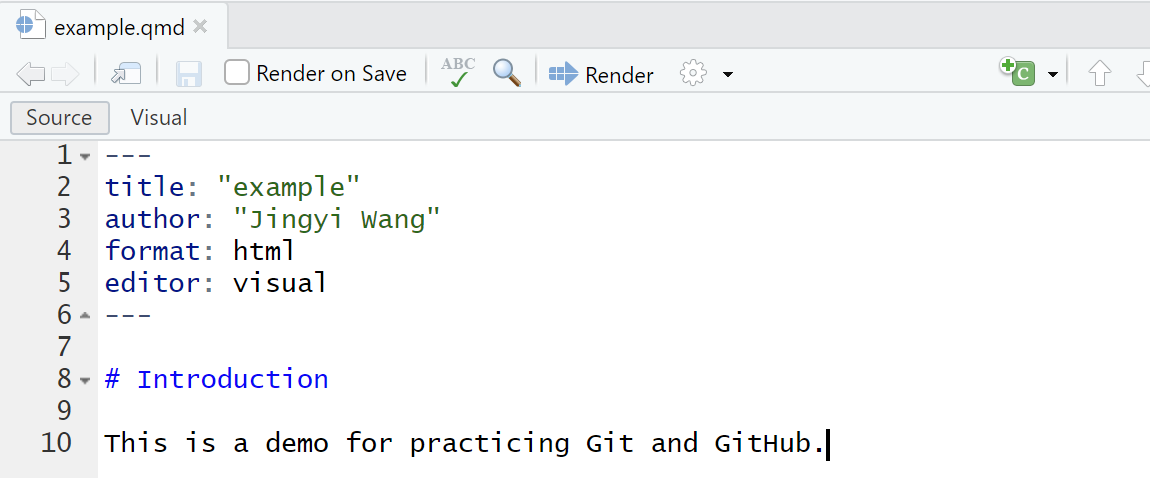
\includegraphics[keepaspectratio]{figure/wri_ex_qmd.png}}

}

\caption{\label{fig-wri_ex_qmd}Write some content}

\end{figure}%

\begin{figure}

\centering{

\pandocbounded{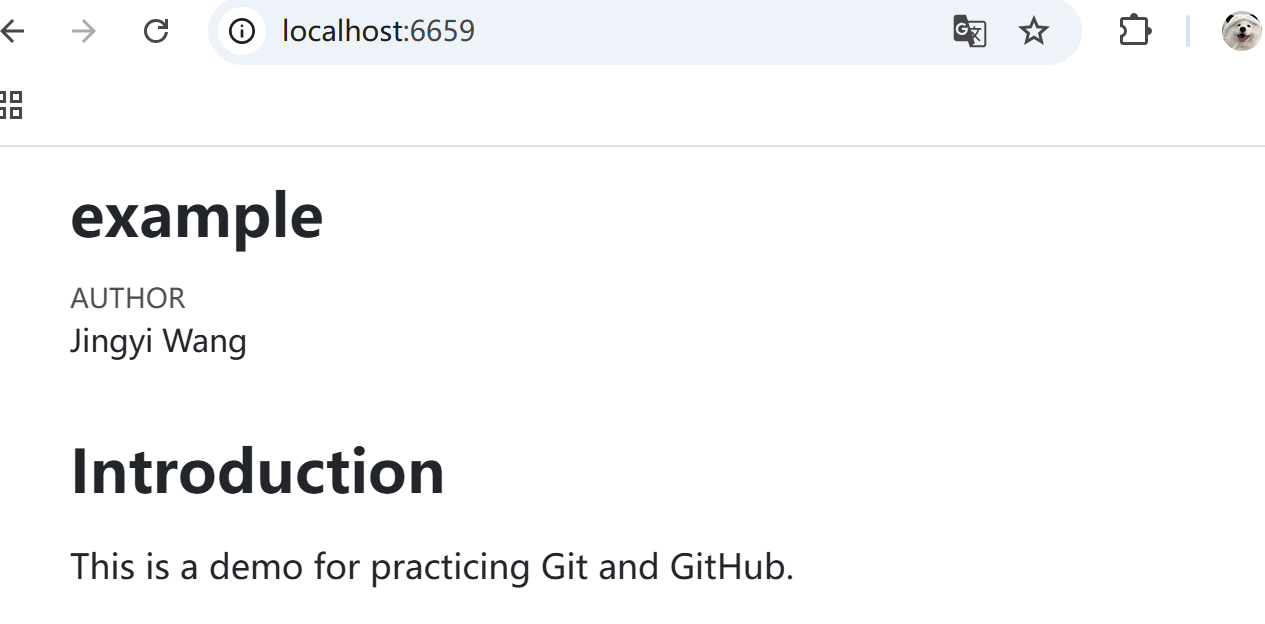
\includegraphics[keepaspectratio]{figure/ex_html.png}}

}

\caption{\label{fig-ex_html}Knit and Create a HTML File}

\end{figure}%

After rendering, your project folder should now contain both the
\texttt{.qmd} file and the \texttt{.html} output
(Figure~\ref{fig-step1_final}).

\begin{figure}

\centering{

\pandocbounded{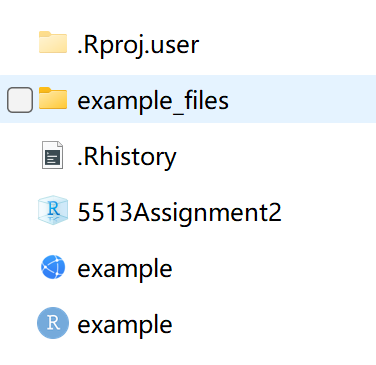
\includegraphics[keepaspectratio]{figure/step1_final.png}}

}

\caption{\label{fig-step1_final}Step1 Final}

\end{figure}%

🧠 \textbf{Reflection:}

This step is important because it sets up your working space. It
connects your folder to Git so it can track changes and link to GitHub
later.

\section{Step 2: Initialize the folder as a Git repository and push to
GitHub}\label{step-2-initialize-the-folder-as-a-git-repository-and-push-to-github}

In RStudio, click the ``Terminal'' tab at the bottom panel, and run the
following commands:

\begin{Shaded}
\begin{Highlighting}[]
\FunctionTok{git}\NormalTok{ init}
\FunctionTok{git}\NormalTok{ add .}
\FunctionTok{git}\NormalTok{ commit }\AttributeTok{{-}m} \StringTok{"Initial commit with example.qmd and knitted HTML"}
\end{Highlighting}
\end{Shaded}

Then, on GitHub, create a new repository (Figure~\ref{fig-new_repo}) and
copy the SSH address(Figure~\ref{fig-SSH}).

\begin{figure}

\centering{

\pandocbounded{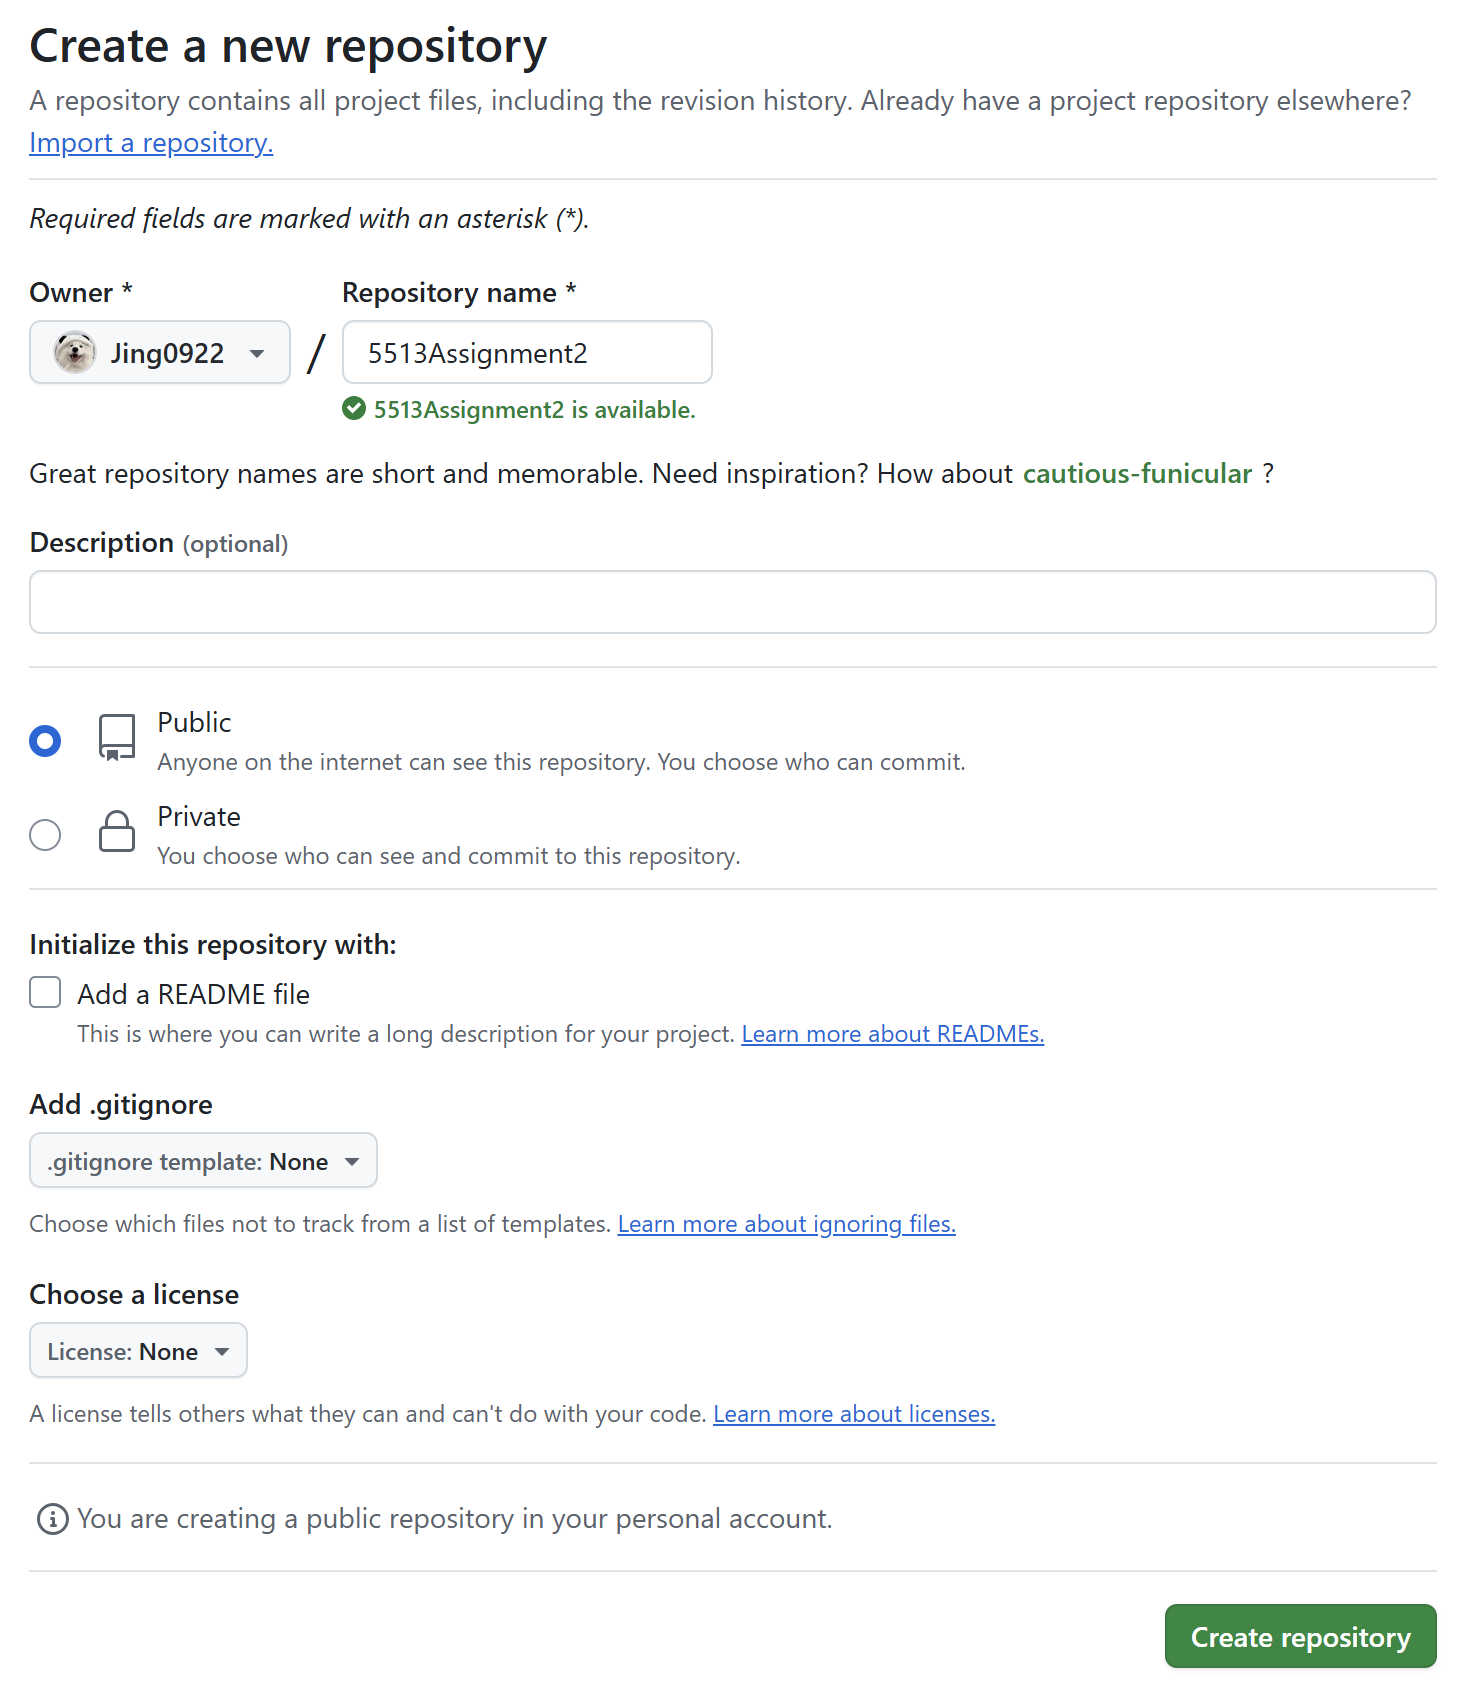
\includegraphics[keepaspectratio]{figure/new_repo.png}}

}

\caption{\label{fig-new_repo}Create a New Repository on GitHub}

\end{figure}%

\begin{figure}

\centering{

\pandocbounded{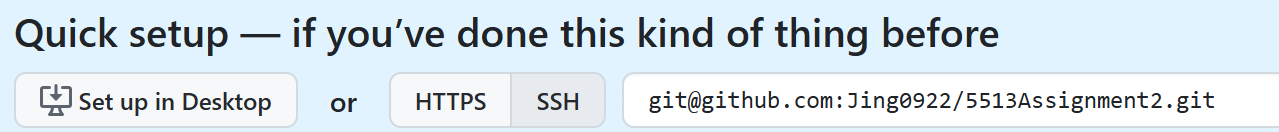
\includegraphics[keepaspectratio]{figure/SSH.png}}

}

\caption{\label{fig-SSH}Copy the SSH}

\end{figure}%

Then link your local repo to GitHub and push it:

\begin{Shaded}
\begin{Highlighting}[]
\FunctionTok{git}\NormalTok{ remote add origin git\textbackslash{}@github.com:Jing0922/5513Assignment2.git}
\FunctionTok{git}\NormalTok{ branch }\AttributeTok{{-}M}\NormalTok{ main}
\FunctionTok{git}\NormalTok{ push }\AttributeTok{{-}u}\NormalTok{ origin main}
\end{Highlighting}
\end{Shaded}

\begin{figure}

\centering{

\pandocbounded{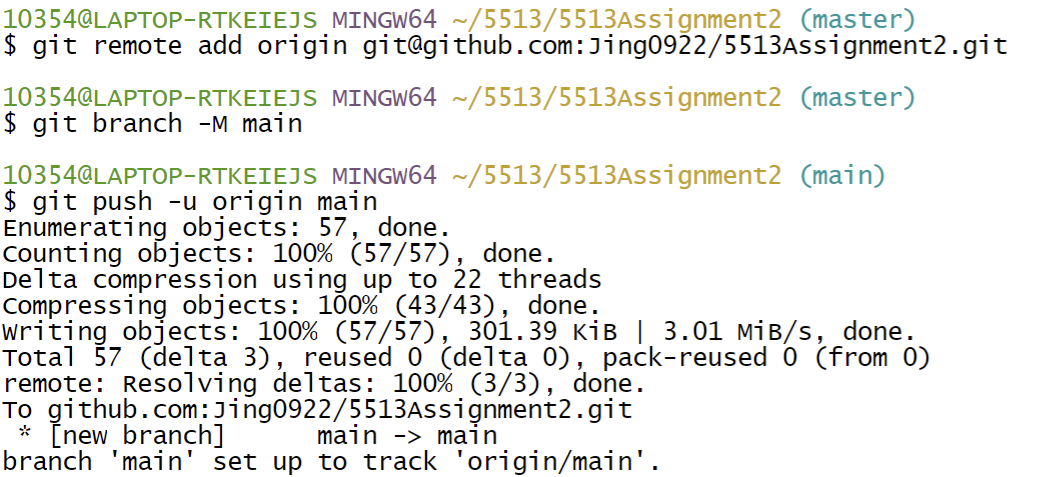
\includegraphics[keepaspectratio]{figure/con_ter.png}}

}

\caption{\label{fig-con_ter}Connect Local Repo to GitHub in Terminal}

\end{figure}%

\begin{figure}

\centering{

\pandocbounded{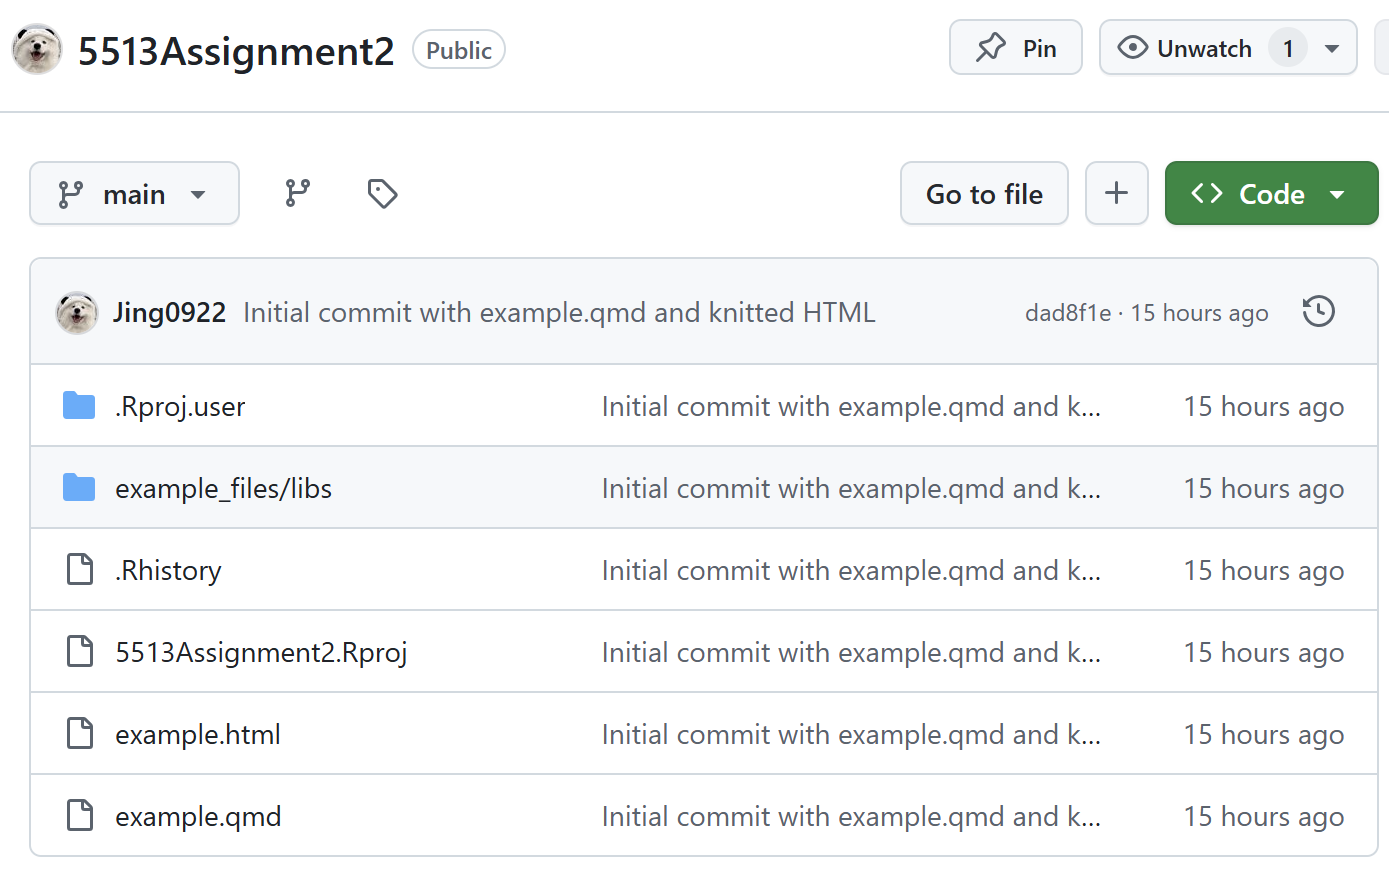
\includegraphics[keepaspectratio]{figure/connect_local_repo.png}}

}

\caption{\label{fig-connect_local_repo}Connect Local Repo to GitHub}

\end{figure}%

🧠 \textbf{What this step does:}

Now your local project is connected to GitHub. You can store your work
online and work with others more easily.

\section{Step 3.1: Create and push a new branch
testbranch}\label{step-3.1-create-and-push-a-new-branch-testbranch}

There are two different ways to create a new branch and move the HEAD to
the new branch:

\begin{enumerate}
\def\labelenumi{\arabic{enumi}.}
\tightlist
\item
  The first method is:
\end{enumerate}

\begin{Shaded}
\begin{Highlighting}[]
\FunctionTok{git}\NormalTok{ branch testbranch}
\FunctionTok{git}\NormalTok{ switch testbranch}
\end{Highlighting}
\end{Shaded}

\begin{enumerate}
\def\labelenumi{\arabic{enumi}.}
\setcounter{enumi}{1}
\tightlist
\item
  Another is:
\end{enumerate}

\begin{Shaded}
\begin{Highlighting}[]
\FunctionTok{git}\NormalTok{ switch }\AttributeTok{{-}c}\NormalTok{ testbranch}
\end{Highlighting}
\end{Shaded}

After any of the above steps,you can check all local branches, use:

\begin{Shaded}
\begin{Highlighting}[]
\FunctionTok{git}\NormalTok{ branch}
\end{Highlighting}
\end{Shaded}

You can see there are two branches
locally(Figure~\ref{fig-create_branch}).

\begin{figure}

\centering{

\pandocbounded{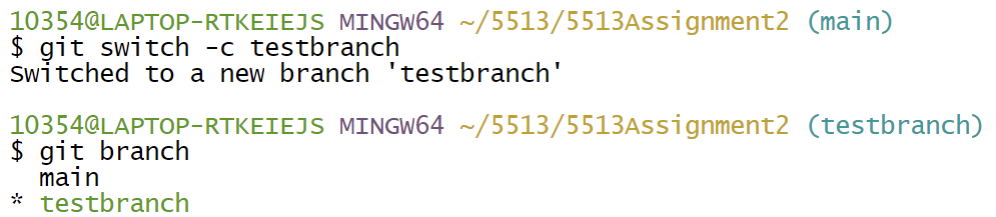
\includegraphics[keepaspectratio]{figure/create_branch.png}}

}

\caption{\label{fig-create_branch}Create testbranch Locally}

\end{figure}%

Now open \texttt{example.qmd}, add a small change (adding a new sentence
on line 11, like Figure~\ref{fig-edit_testbranch_qmd}), and save it.

\begin{figure}

\centering{

\pandocbounded{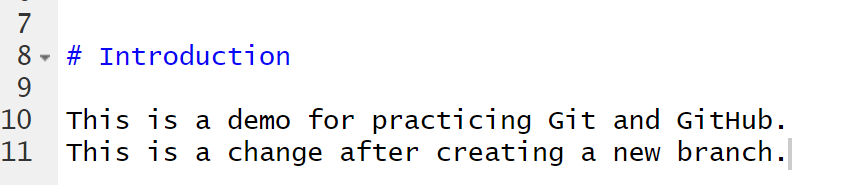
\includegraphics[keepaspectratio]{figure/edit_testbranch_qmd.png}}

}

\caption{\label{fig-edit_testbranch_qmd}Edit example.qmd in testbranch}

\end{figure}%

Then run these commands:

\begin{Shaded}
\begin{Highlighting}[]
\FunctionTok{git}\NormalTok{ add example.qmd}
\FunctionTok{git}\NormalTok{ commit }\AttributeTok{{-}m} \StringTok{"Edit example.qmd in testbranch"}
\FunctionTok{git}\NormalTok{ push origin testbranch}
\end{Highlighting}
\end{Shaded}

The result is shown in Figure~\ref{fig-git_push_testbranch}.

\begin{figure}

\centering{

\pandocbounded{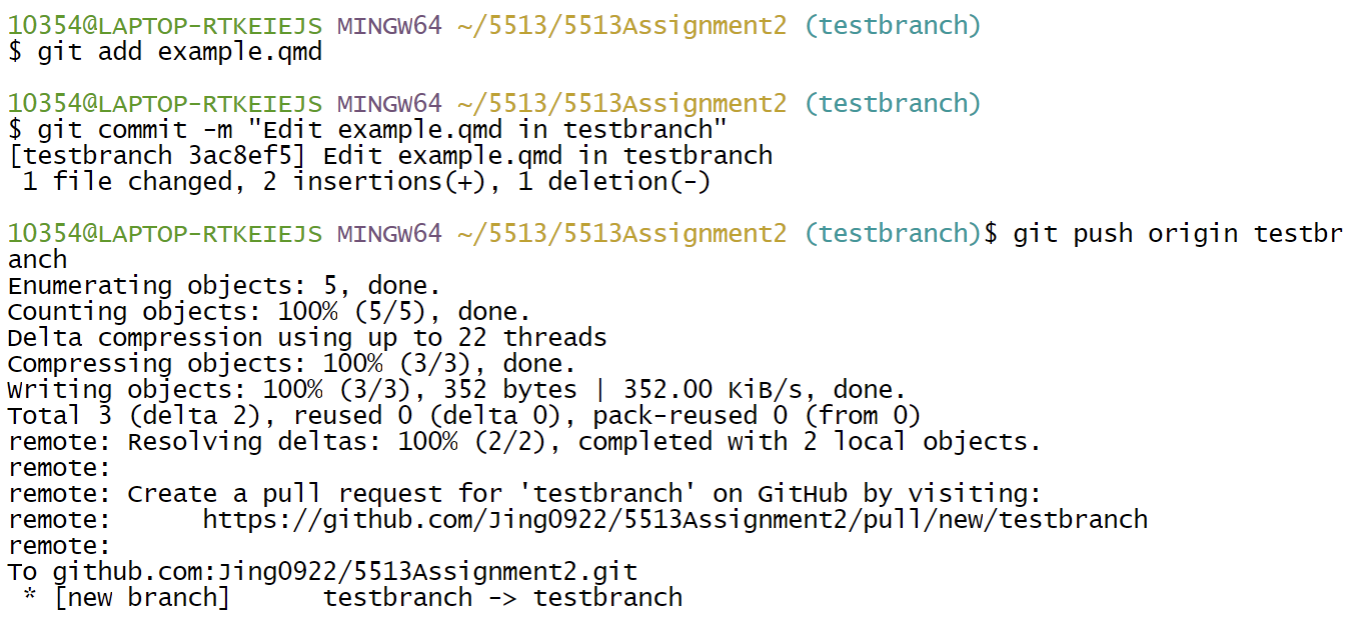
\includegraphics[keepaspectratio]{figure/git_push_testbranch.png}}

}

\caption{\label{fig-git_push_testbranch}Add, Commit and Push example.qmd
in testbranch}

\end{figure}%

🧠 \textbf{Why use branches?}

Branches let you test new ideas without changing your main files. This
keeps your main project safe.

\section{Step 3.2: create a folder called
data}\label{step-3.2-create-a-folder-called-data}

Now still in \texttt{testbranch}, we want to create a new folder and add
the data from Assignment 1 to it(Figure~\ref{fig-data}). In the
terminal, you can use this command to make a folder:

\begin{Shaded}
\begin{Highlighting}[]
\FunctionTok{mkdir}\NormalTok{ data}
\end{Highlighting}
\end{Shaded}

To copy the data file, you have two options:

\begin{enumerate}
\def\labelenumi{\arabic{enumi}.}
\tightlist
\item
  Using Git bash, may not always work:
\end{enumerate}

\begin{Shaded}
\begin{Highlighting}[]
\FunctionTok{cp} \StringTok{"/c/Users/10354/5513/etc5513{-}assignment{-}1{-}Jing0922/Data/Meat\_con.csv"} \StringTok{"./data/"}
\end{Highlighting}
\end{Shaded}

\begin{enumerate}
\def\labelenumi{\arabic{enumi}.}
\setcounter{enumi}{1}
\tightlist
\item
  Safer way: Just manually copy the file into the data folder using File
  Explorer.
\end{enumerate}

\begin{figure}

\centering{

\pandocbounded{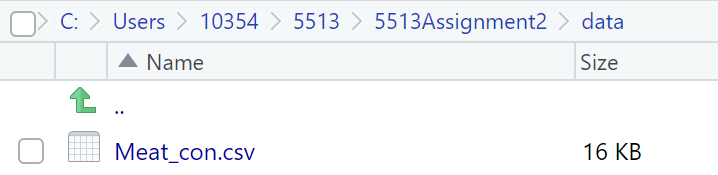
\includegraphics[keepaspectratio]{figure/data.png}}

}

\caption{\label{fig-data}Create a New Folder and Copy the Data}

\end{figure}%

Now add and commit the changes:

\begin{Shaded}
\begin{Highlighting}[]
\FunctionTok{git}\NormalTok{ add data/}
\FunctionTok{git}\NormalTok{ commit }\AttributeTok{{-}m} \StringTok{"Add data folder with assignment 1 data"}
\end{Highlighting}
\end{Shaded}

The final result is shown in Figure~\ref{fig-data_create_copy_commit}.

\begin{figure}

\centering{

\pandocbounded{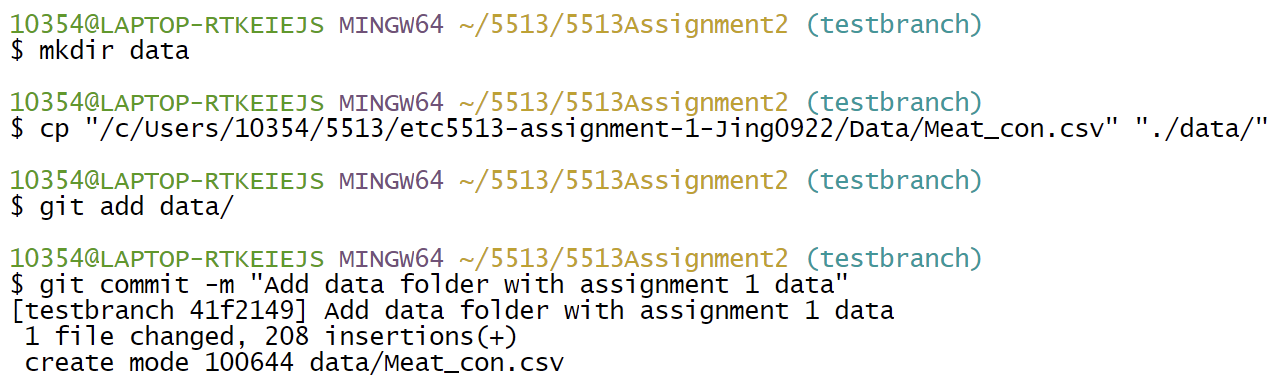
\includegraphics[keepaspectratio]{figure/data_create_copy_commit.png}}

}

\caption{\label{fig-data_create_copy_commit}Add and Commit the Changes}

\end{figure}%

🧠 \textbf{What did we do?}

We saved useful data in the repo and tracked it with Git.

\section{Step 4: Amend the previous
commit}\label{step-4-amend-the-previous-commit}

Sometimes we forget to include something in the last commit. We can fix
that with \texttt{-\/-amend}.

First, check the commit history:

\begin{Shaded}
\begin{Highlighting}[]
\FunctionTok{git}\NormalTok{ log }\AttributeTok{{-}{-}oneline}
\end{Highlighting}
\end{Shaded}

You will get three commits now(Figure~\ref{fig-log_his_1}).

\begin{figure}

\centering{

\pandocbounded{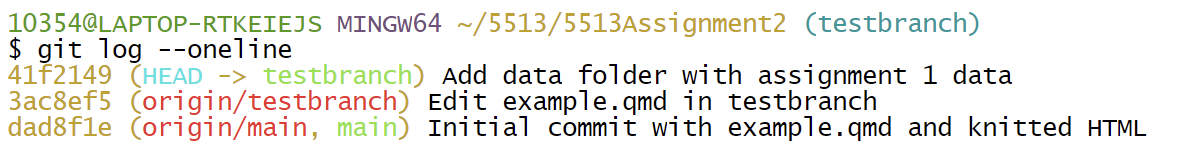
\includegraphics[keepaspectratio]{figure/log_his_1.png}}

}

\caption{\label{fig-log_his_1}Check the Commit History}

\end{figure}%

Then:

\begin{Shaded}
\begin{Highlighting}[]
\FunctionTok{git}\NormalTok{ commit }\AttributeTok{{-}{-}amend}
\end{Highlighting}
\end{Shaded}

This will open the Vim editor (Figure~\ref{fig-Vim_editor}) showing the
last commit message.

💡 \textbf{Vim Tip}: If you're new to Vim, remember:

\begin{itemize}
\tightlist
\item
  Press i to enter Insert mode (cursor starts blinking)
\item
  Modify the message as needed
\item
  Press Esc to return to Command mode
\item
  Type :wq then press Enter to: write (save) + quit (exit Vim)
\end{itemize}

\begin{figure}

\centering{

\pandocbounded{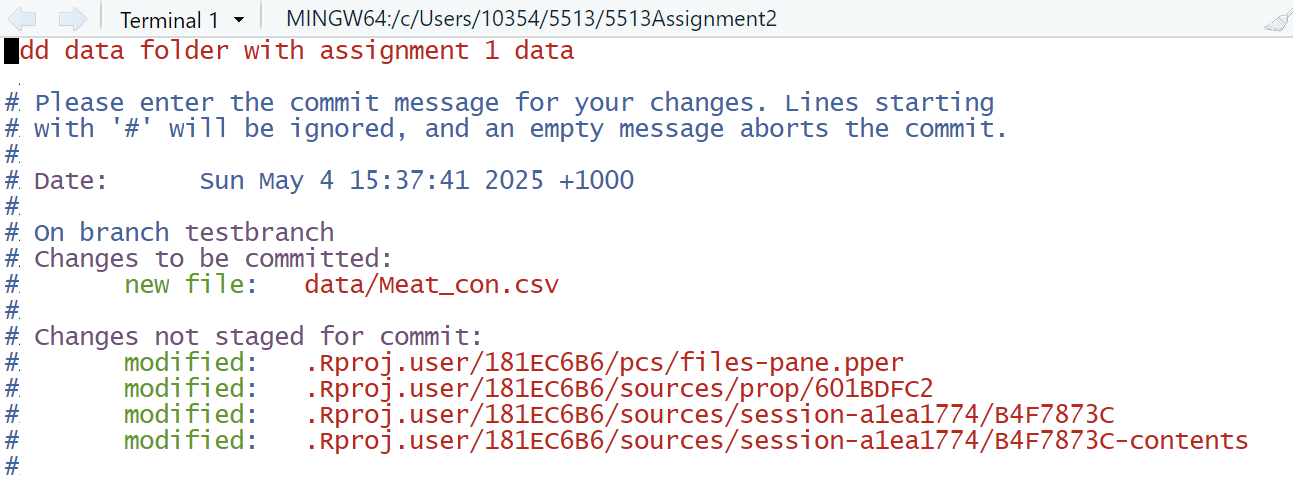
\includegraphics[keepaspectratio]{figure/Vim_editor.png}}

}

\caption{\label{fig-Vim_editor}Vim Editor}

\end{figure}%

\begin{figure}

\centering{

\pandocbounded{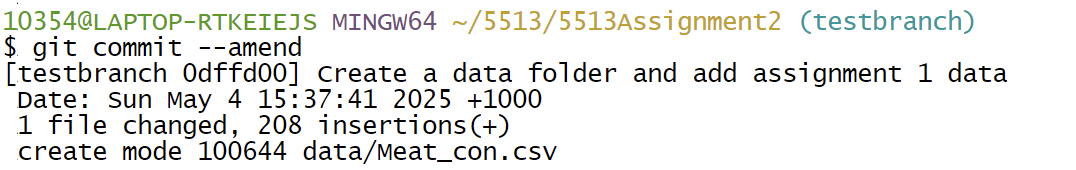
\includegraphics[keepaspectratio]{figure/amend.png}}

}

\caption{\label{fig-amend}Amend the Last Commit Message}

\end{figure}%

After editing, run:

\begin{Shaded}
\begin{Highlighting}[]
\FunctionTok{git}\NormalTok{ push origin testbranch }\AttributeTok{{-}{-}force}
\end{Highlighting}
\end{Shaded}

Now you check the commit history again:

\begin{Shaded}
\begin{Highlighting}[]
\FunctionTok{git}\NormalTok{ log }\AttributeTok{{-}{-}oneline}
\end{Highlighting}
\end{Shaded}

You can see that the last commit has been
modified(Figure~\ref{fig-log_his_2}).

\begin{figure}

\centering{

\pandocbounded{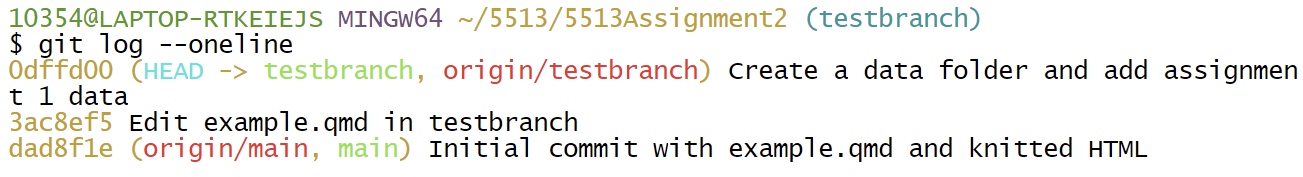
\includegraphics[keepaspectratio]{figure/log_his_2.png}}

}

\caption{\label{fig-log_his_2}Check the Commit History after Amending}

\end{figure}%

🧠 \textbf{Why use --amend?}

It lets us fix the last commit instead of making a new one.

\begin{longtable}[]{@{}lll@{}}
\toprule\noalign{}
Command & Use Case & Safety \\
\midrule\noalign{}
\endhead
\bottomrule\noalign{}
\endlastfoot
\texttt{git\ commit\ -\/-amend} & Edit the \textbf{most recent commit} &
Medium \\
\texttt{git\ reset} & Rewind to \textbf{any past commit} & High \\
\end{longtable}

🧠 \textbf{Why use --force?}

Because the history changed, GitHub needs a forced update to accept it.

⚠️ \textbf{Warning:}

Amending rewrites Git history. After \texttt{amend}, you must use
\texttt{git\ push\ -f}. This is \textbf{dangerous} if others are working
on the same branch! Always check with your team first.

\section{Step 5: Switch back to the main branch and cause a merge
conflict}\label{step-5-switch-back-to-the-main-branch-and-cause-a-merge-conflict}

Now we go back to the main branch:

\begin{Shaded}
\begin{Highlighting}[]
\FunctionTok{git}\NormalTok{ checkout main}
\end{Highlighting}
\end{Shaded}

Notice that the changes of \texttt{example.qmd} made in
\texttt{testbranch} (the line 11 modification shown in
Figure~\ref{fig-edit_testbranch_qmd}) are now absent. \textbf{Don't be
worried!} This is expected behavior when switching branches.

Now, we deliberately create a conflict. Open \texttt{example.qmd} and
edit the same line 11 (but with different content than in
\texttt{testbranch}). And add new content to other lines (as shown in
Figure~\ref{fig-edit_main_qmd}). Save it.

\begin{figure}

\centering{

\pandocbounded{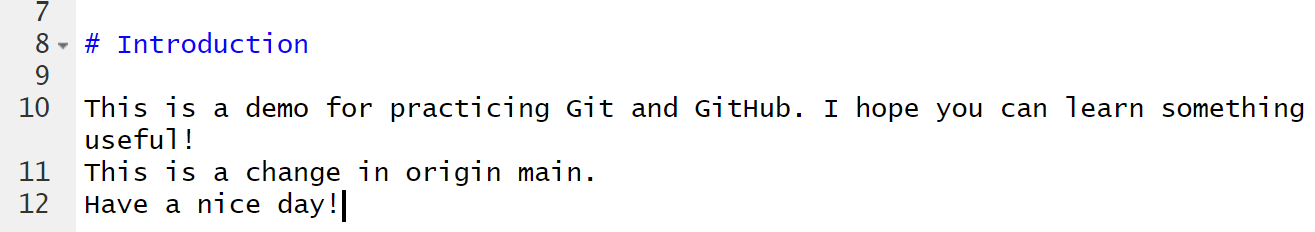
\includegraphics[keepaspectratio]{figure/edit_main_qmd.png}}

}

\caption{\label{fig-edit_main_qmd}Edit example.qmd in main}

\end{figure}%

Then run:

\begin{Shaded}
\begin{Highlighting}[]
\FunctionTok{git}\NormalTok{ add example.qmd}
\FunctionTok{git}\NormalTok{ commit }\AttributeTok{{-}m} \StringTok{"Conflicting change in main branch"}
\FunctionTok{git}\NormalTok{ push origin main}
\end{Highlighting}
\end{Shaded}

\begin{figure}

\centering{

\pandocbounded{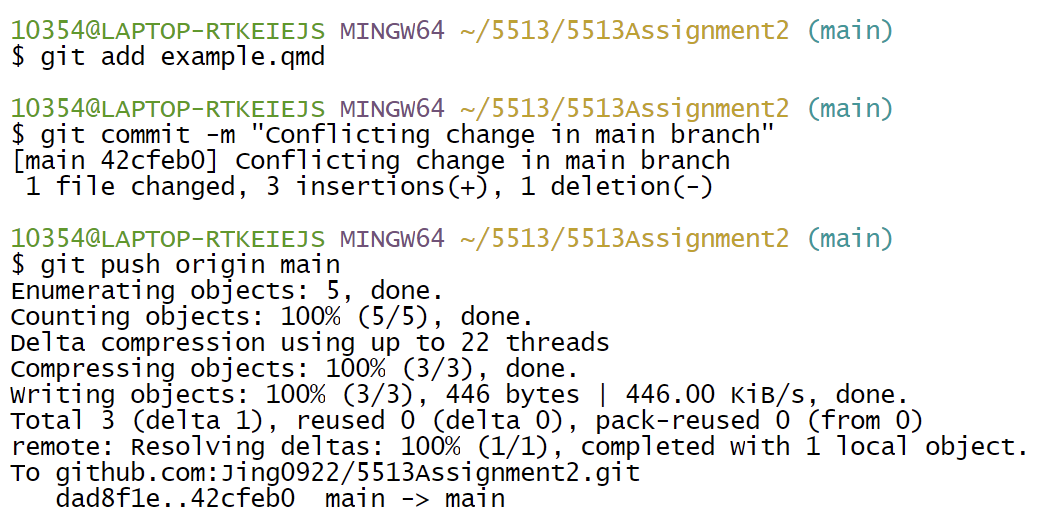
\includegraphics[keepaspectratio]{figure/git_push_main.png}}

}

\caption{\label{fig-git_push_main}Add, Commit and Push example.qmd in
main}

\end{figure}%

🧠 \textbf{Why do this?}

We're preparing for a merge conflict by changing the same line in two
branches.

\section{Step 6: Merge testbranch into main and resolve
conflict}\label{step-6-merge-testbranch-into-main-and-resolve-conflict}

Now we try to combine the two branches:

\begin{Shaded}
\begin{Highlighting}[]
\FunctionTok{git}\NormalTok{ merge testbranch}
\end{Highlighting}
\end{Shaded}

⚠️ \textbf{Critical Check:}

You \emph{must} be on the \texttt{main} branch before merging. If you
accidentally run \texttt{git\ merge\ main} while on \texttt{testbranch},
the merge direction will be reversed!

A conflict will appear in \texttt{example.qmd}. It looks like
Figure~\ref{fig-merge_conflict}. There are a lot of markers, such as
\textless\textless\textless\textless\textless\textless\textless, =======
and
\textgreater\textgreater\textgreater\textgreater\textgreater\textgreater\textgreater.

\begin{figure}

\centering{

\pandocbounded{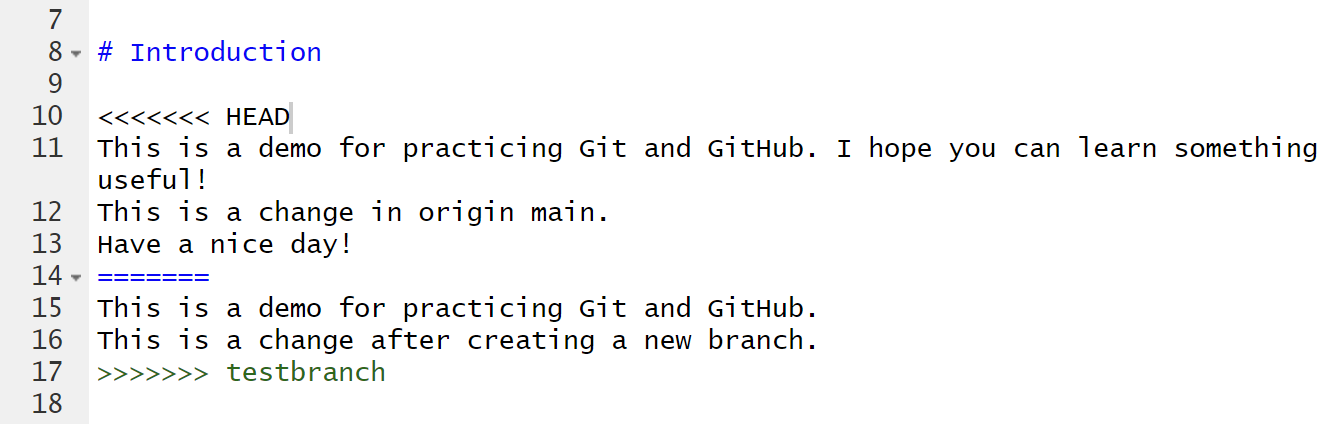
\includegraphics[keepaspectratio]{figure/merge_conflict.png}}

}

\caption{\label{fig-merge_conflict}A Conflict when Combine Two Branch}

\end{figure}%

Open the file and manually fix the content. You can keep both lines,
delete one, or rewrite(Figure~\ref{fig-resolve_conflict}). Save it.

\begin{figure}

\centering{

\pandocbounded{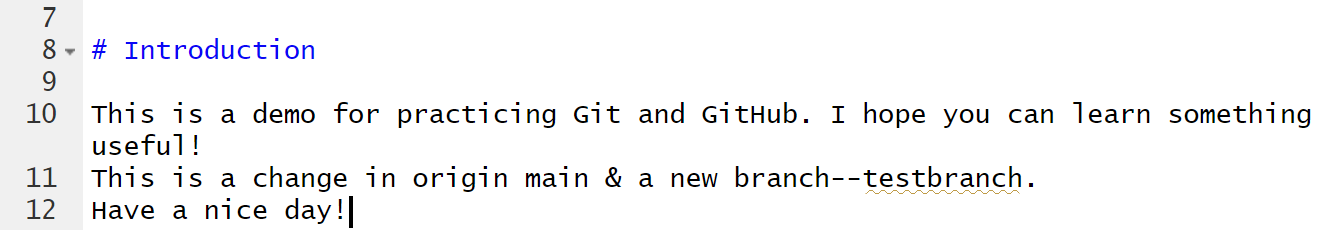
\includegraphics[keepaspectratio]{figure/resolve_conflict.png}}

}

\caption{\label{fig-resolve_conflict}Resolve Conflict}

\end{figure}%

Then:

\begin{Shaded}
\begin{Highlighting}[]
\FunctionTok{git}\NormalTok{ add example.qmd}
\FunctionTok{git}\NormalTok{ commit }\AttributeTok{{-}m} \StringTok{"Resolve merge conflict"}
\FunctionTok{git}\NormalTok{ push origin main}
\end{Highlighting}
\end{Shaded}

To check status:

\begin{Shaded}
\begin{Highlighting}[]
\FunctionTok{git}\NormalTok{ status}
\end{Highlighting}
\end{Shaded}

The result is Figure~\ref{fig-after_merge_local}. In GitHub, the
\texttt{example.qmd} looks like Figure~\ref{fig-after_merge_qmd}.

\begin{figure}

\centering{

\pandocbounded{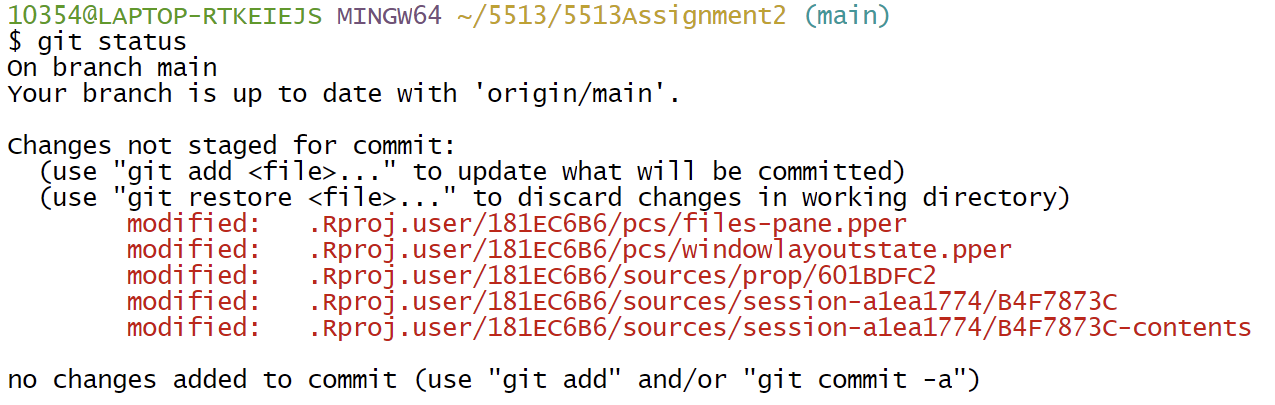
\includegraphics[keepaspectratio]{figure/after_merge_local.png}}

}

\caption{\label{fig-after_merge_local}The Status after Resolving
Conflict Locally}

\end{figure}%

\begin{figure}

\centering{

\pandocbounded{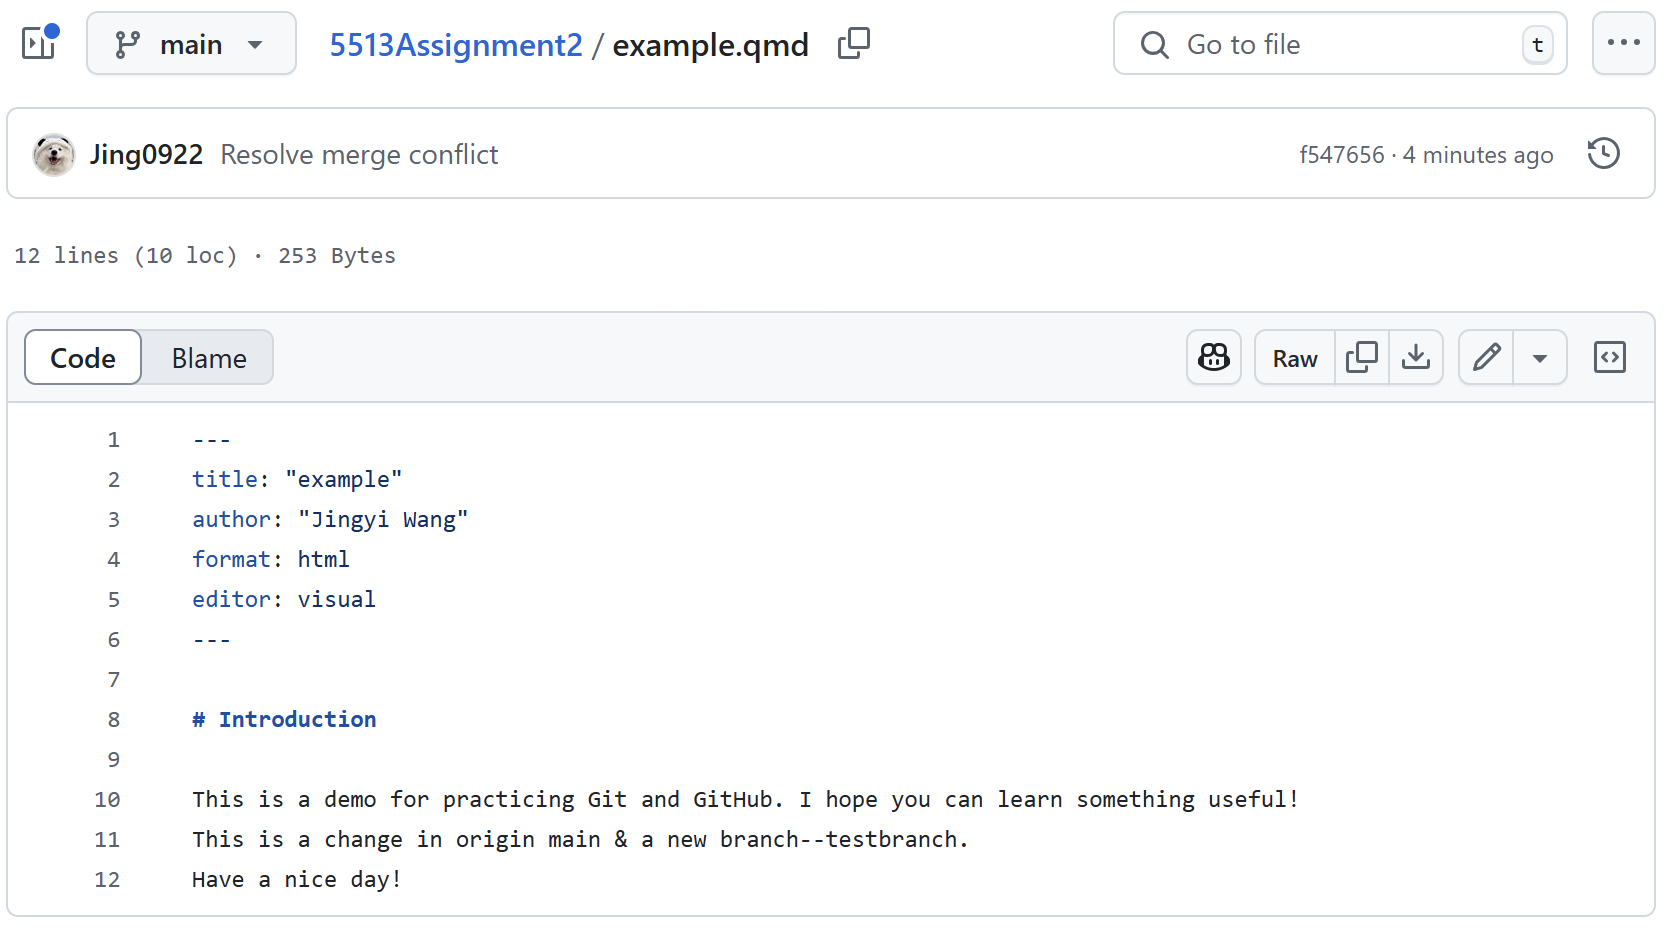
\includegraphics[keepaspectratio]{figure/after_merge_qmd.png}}

}

\caption{\label{fig-after_merge_qmd}The example.qmd after Resolving
Conflict in GitHub}

\end{figure}%

🧠 \textbf{Why do conflicts happen?}

Conflicts happen when both branches edit the same lines. Git needs your
help to resolve it.

🧠 \textbf{Why we do this:}

Merging brings together updates from different branches. It's a key part
of collaboration and ensures everyone's work fits together.

\section{Step 7: Tag the commit as version
1.0}\label{step-7-tag-the-commit-as-version-1.0}

Now we want to mark the current commit as a version.

Use this command to create an annotated tag:

\begin{Shaded}
\begin{Highlighting}[]
\FunctionTok{git}\NormalTok{ tag }\AttributeTok{{-}a}\NormalTok{ v1.0 }\AttributeTok{{-}m} \StringTok{"Release version 1.0"}
\FunctionTok{git}\NormalTok{ push origin v1.0}
\end{Highlighting}
\end{Shaded}

This creates a tag named ``v1.0'', which will appear on
GitHub(Figure~\ref{fig-tag_on_github}).

\begin{figure}

\centering{

\pandocbounded{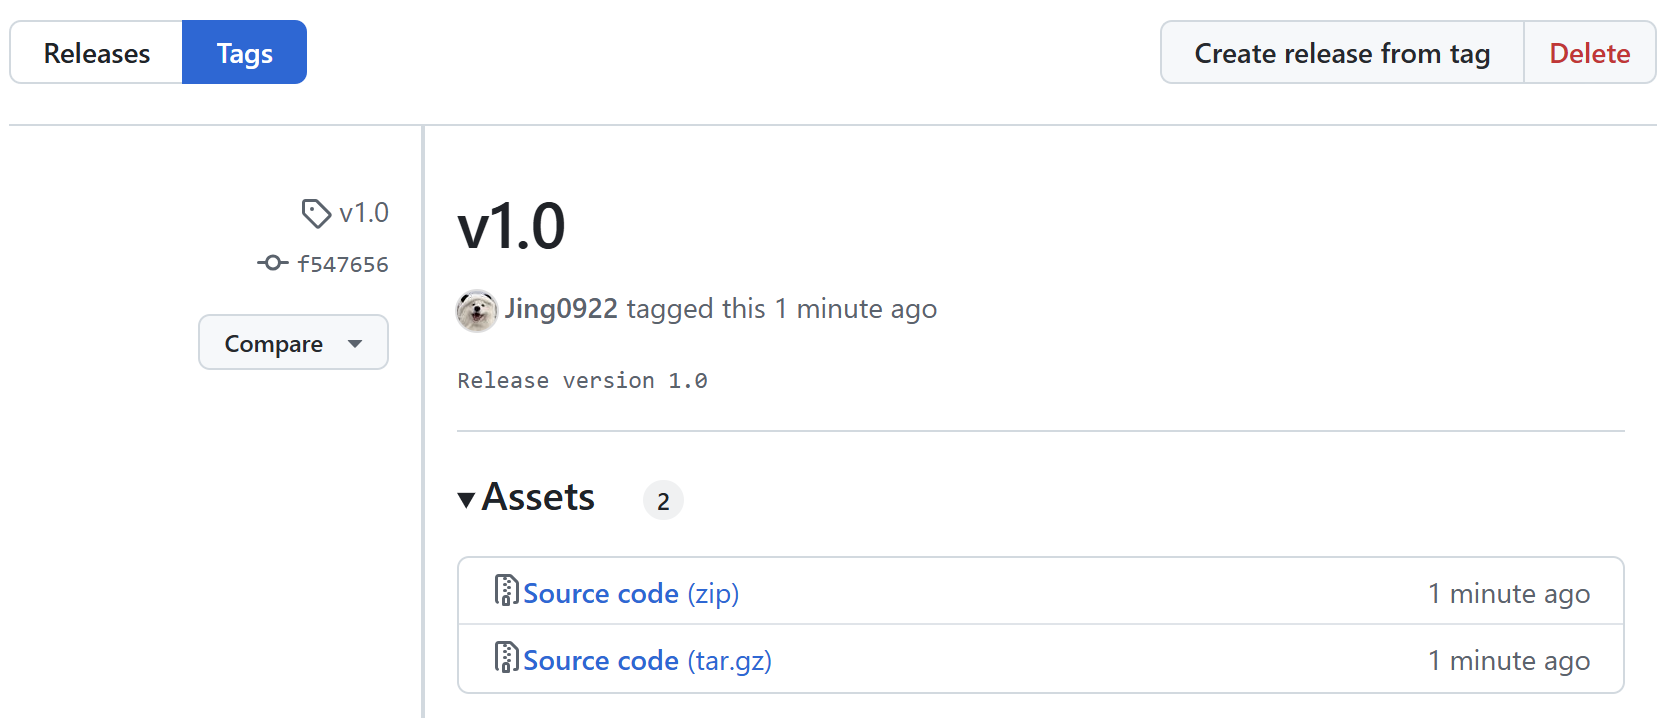
\includegraphics[keepaspectratio]{figure/tag_on_github.png}}

}

\caption{\label{fig-tag_on_github}Create an Annotated Tag}

\end{figure}%

🧠 \textbf{Reminder:}

Tags are like bookmarks. They help you find key points in your project
history. Annotated tags (-a) store extra metadata including who created
them and when.

\section{Step 8: Delete the
testbranch}\label{step-8-delete-the-testbranch}

Now that testbranch has been successfully merged into main, we can
safely remove it to keep our repository organized.

⚠️ \textbf{Critical Check:}

You can not delete your currently active branch, which means you
\emph{can not} be on the \texttt{testbranch}.

Delete the branch locally:

\begin{Shaded}
\begin{Highlighting}[]
\FunctionTok{git}\NormalTok{ branch }\AttributeTok{{-}d}\NormalTok{ testbranch }
\end{Highlighting}
\end{Shaded}

Check branch, use:

\begin{Shaded}
\begin{Highlighting}[]
\FunctionTok{git}\NormalTok{ branch}
\end{Highlighting}
\end{Shaded}

Delete the branch from GitHub (remote):

\begin{Shaded}
\begin{Highlighting}[]
\FunctionTok{git}\NormalTok{ push origin }\AttributeTok{{-}{-}delete}\NormalTok{ testbranch}
\end{Highlighting}
\end{Shaded}

Now, only the main branch will be left
locally(Figure~\ref{fig-delete_branch_local}) and in your GitHub
repo(Figure~\ref{fig-delete_branch_github}).

\begin{figure}

\centering{

\pandocbounded{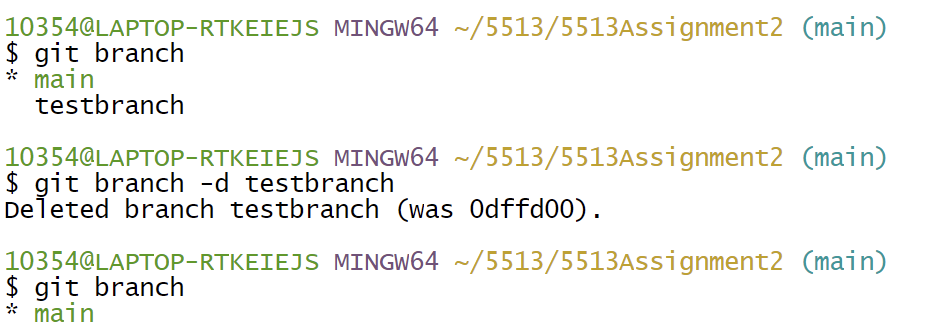
\includegraphics[keepaspectratio]{figure/delete_branch_local.png}}

}

\caption{\label{fig-delete_branch_local}Delete the Branch Locally}

\end{figure}%

\begin{figure}

\centering{

\pandocbounded{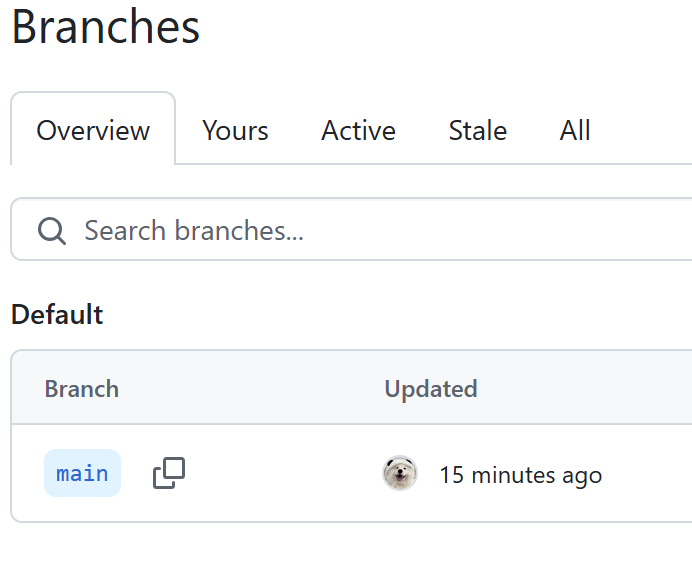
\includegraphics[keepaspectratio]{figure/delete_branch_github.png}}

}

\caption{\label{fig-delete_branch_github}Delete the Branch from GitHub}

\end{figure}%

🧠 \textbf{Why delete branches?}

Deleting old branches keeps your project tidy and organized. Just
remember: Git won't let you delete the branch you're currently using.

\section{Step 9: View the commit log}\label{step-9-view-the-commit-log}

You can check the history of your changes by using:

\begin{Shaded}
\begin{Highlighting}[]
\FunctionTok{git}\NormalTok{ log }\AttributeTok{{-}{-}oneline}
\end{Highlighting}
\end{Shaded}

This shows a short list of all your commits with commit IDs and
messages(Figure~\ref{fig-log_his_3}).

\begin{figure}

\centering{

\pandocbounded{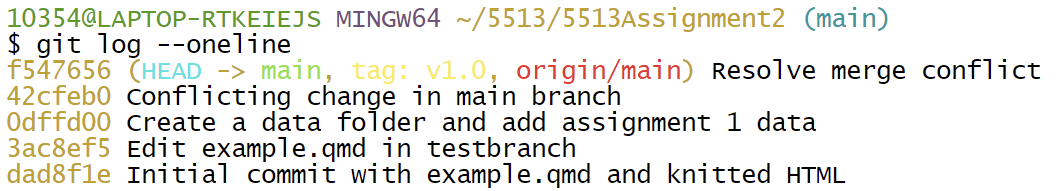
\includegraphics[keepaspectratio]{figure/log_his_3.png}}

}

\caption{\label{fig-log_his_3}Check the Commit History}

\end{figure}%

🧠 \textbf{Why do this?}

Viewing the commit history shows who made changes, when, and what was
done. It's especially helpful for tracking team work or reviewing your
progress.

\section{Step 10: Add a plot and undo a
commit}\label{step-10-add-a-plot-and-undo-a-commit}

Add a new section to \texttt{example.qmd} and draw a plot, like
Figure~\ref{fig-add_plot}.

\begin{figure}

\centering{

\pandocbounded{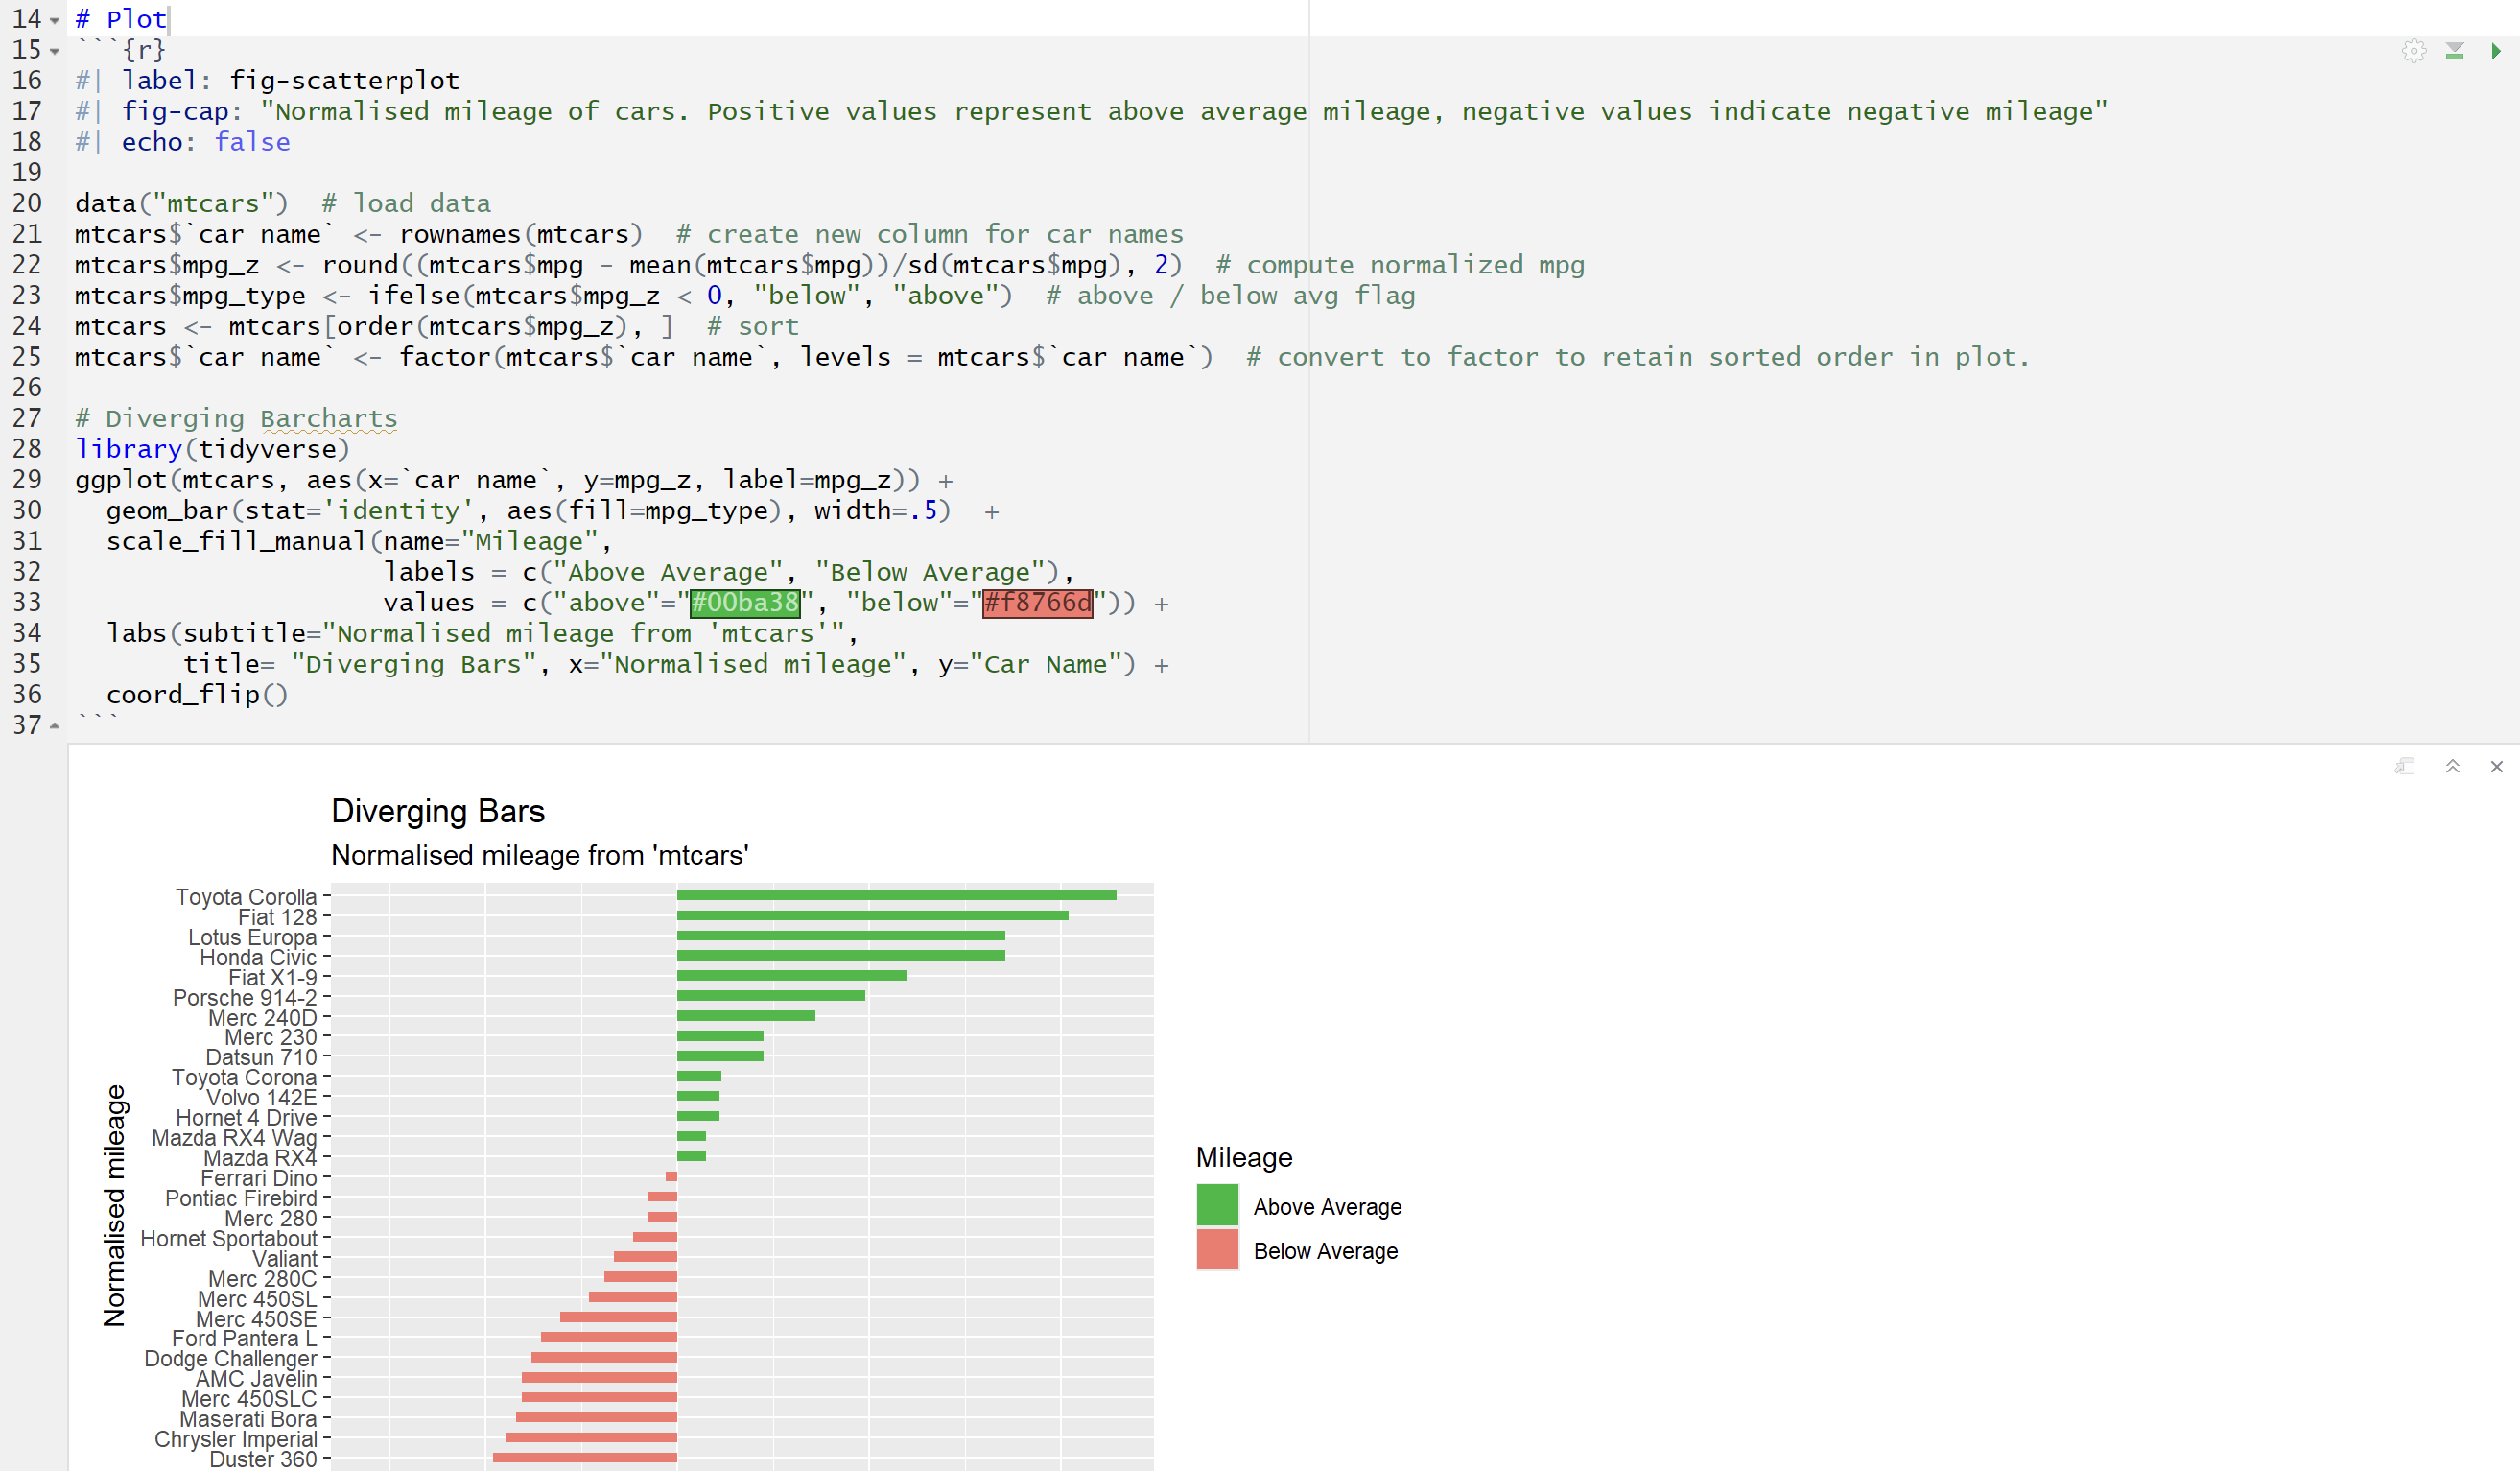
\includegraphics[keepaspectratio]{figure/add_plot.png}}

}

\caption{\label{fig-add_plot}Add the Plot}

\end{figure}%

Then add and commit it:

\begin{Shaded}
\begin{Highlighting}[]
\FunctionTok{git}\NormalTok{ add example.qmd}
\FunctionTok{git}\NormalTok{ commit }\AttributeTok{{-}m} \StringTok{"Add simple plot"}
\end{Highlighting}
\end{Shaded}

To undo the most recent commit but keep all changes in your working
directory, use a \textbf{soft reset}:

\begin{Shaded}
\begin{Highlighting}[]
\FunctionTok{git}\NormalTok{ reset }\AttributeTok{{-}{-}soft}\NormalTok{ HEAD\textasciitilde{}1}
\end{Highlighting}
\end{Shaded}

This command removes the last commit but keeps the changes in the
staging area.

To verify the changes:

\begin{Shaded}
\begin{Highlighting}[]
\FunctionTok{git}\NormalTok{ status}
\end{Highlighting}
\end{Shaded}

You can see that all previously committed changes now appear as
``Changes to be committed'' (shown in
green)(Figure~\ref{fig-reset_soft_status})

\begin{figure}

\centering{

\pandocbounded{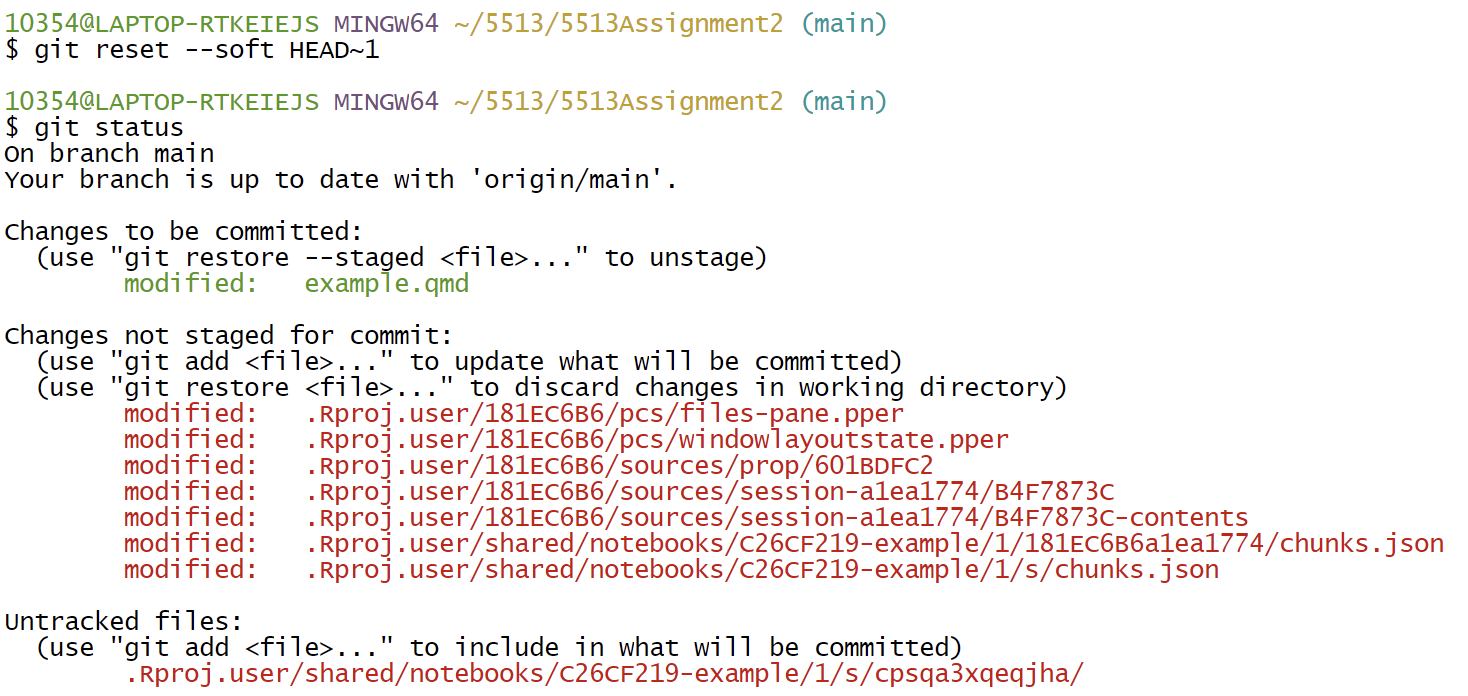
\includegraphics[keepaspectratio]{figure/reset_soft_status.png}}

}

\caption{\label{fig-reset_soft_status}The Status after Soft Reset}

\end{figure}%

🧠 \textbf{Why do this?}

Sometimes we want to fix a commit message or add more things before
pushing it. Soft reset is useful when you want to change the commit
message or add more to the commit.

\textbf{Extended Knowledge: Other Reset Modes}

\textbf{Mixed Reset(Default)}

\begin{Shaded}
\begin{Highlighting}[]
\FunctionTok{git}\NormalTok{ reset HEAD\textasciitilde{}1}
\end{Highlighting}
\end{Shaded}

This command unstages changes but keeps them in working directory. If
you verify with git status, changes show as unstaged in red.

\textbf{Hard Reset(⚠️ Dangerous!)}

\begin{Shaded}
\begin{Highlighting}[]
\FunctionTok{git}\NormalTok{ reset }\AttributeTok{{-}{-}hard}\NormalTok{ HEAD\textasciitilde{}1}
\end{Highlighting}
\end{Shaded}

This command completely discards the commit and \textbf{all} local
changes. No recovery unless you used git reflog.

🧠 \textbf{Be careful:}

\begin{enumerate}
\def\labelenumi{\arabic{enumi}.}
\tightlist
\item
  Soft reset (--soft) → Keeps changes staged.
\item
  Mixed reset (--mixed) → Keeps changes but unstages them.
\item
  Hard reset (--hard) → Deletes everything in the commit.
\end{enumerate}

\section{Tips}\label{tips}

There are some tips for you:

\begin{itemize}
\item
  Use clear commit messages like ``Add plot section to qmd'' or ``Fix
  conflict between branches''.
\item
  Keep commits small and focused.
\item
  Always use branches when testing or adding new features.
\end{itemize}

\section{Conclusion}\label{conclusion}

This guide gives you a strong start with Git, GitHub, RStudio and CLI.
By learning these steps, you can manage your work more clearly and work
better with others.




\end{document}
